% !TeX root = Protokoll.tex
Der größte Anteil aller Festkörper, besitzt einen kristallinen Aufbau. Dies bedeutet die Atome sind räumlich periodisch angeordnet. Um die Kristalleigenschaften zu diskutieren wird ein einzelner Kristall oder auch Einkristall betrachtet, weil sich die anisotropen Eigenschaften in Kristallen die sich im polykristallinem Zustand befinden heraus Mitteln. Um Kristalle Vermessen zu können, werden Strahlen benötigt deren Wellenlänge sich in der Größenordnung des Atomabstands befinden. Bei der Dybe-Scherrer-Methode werden dafür Röntgenstrahlen verwendet.
\subsection{Kristallstrukturen}
\begin{figure}[h!]
	\centering
	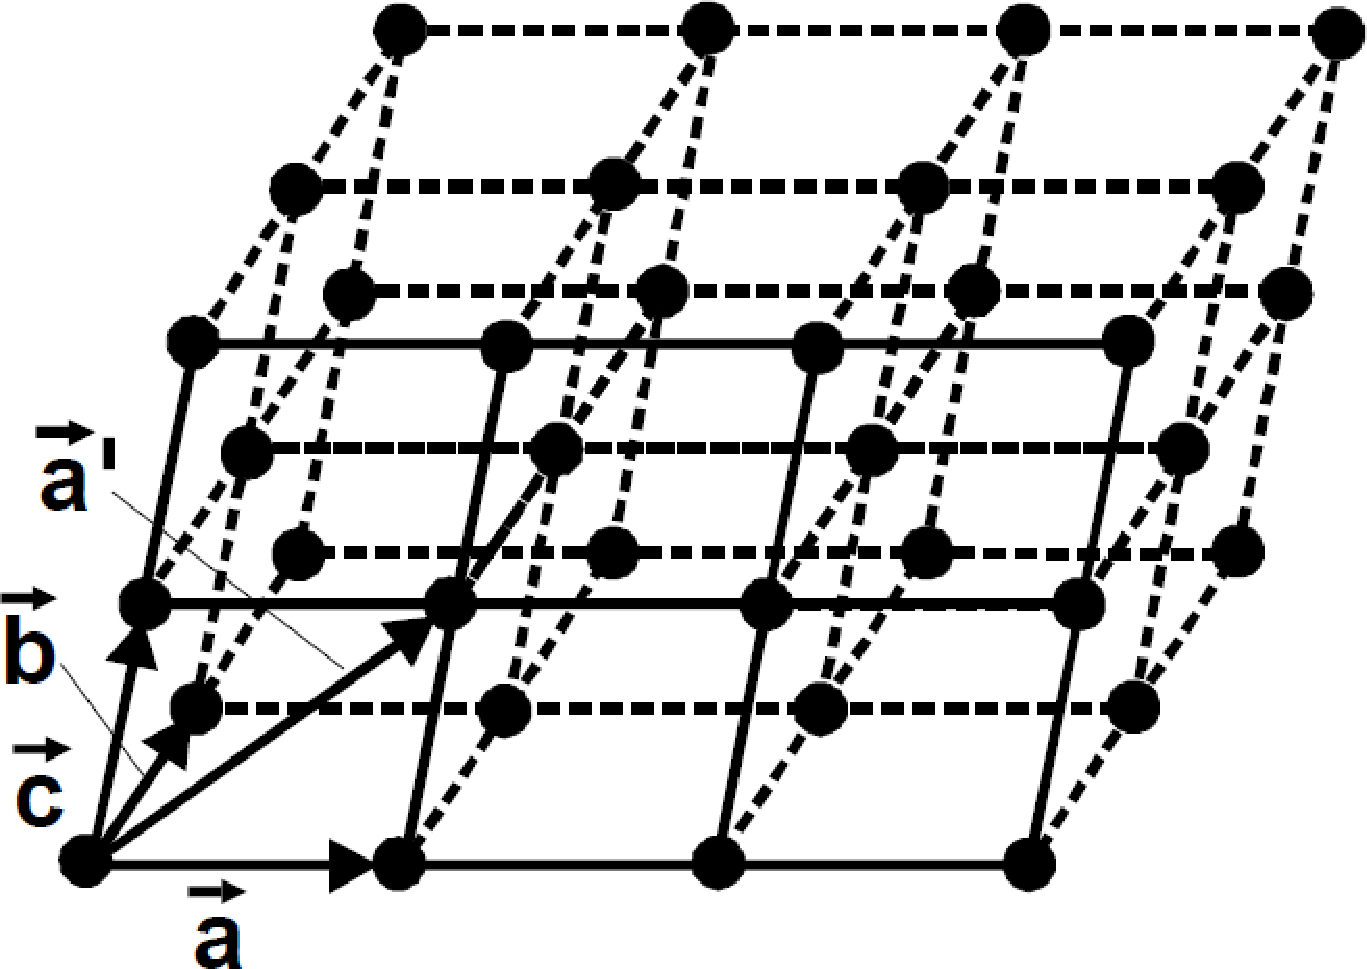
\includegraphics[scale = 0.4]{../Grafiken/Gitter.pdf}
	\caption{Eine Veranschaulichung für ein Kristallgitter.\cite{V41}}
	\label{fig:BeispielGitter}
\end{figure}
Ein Kristall kann als dreidimensionales Gitter beschrieben werden. Die Eckpunkte sind die Basis und beschreiben die Positionen der Atome oder von Atomgruppen.
Aufgrund der Periodizität des Kristalls, lässt er sich vollständig durch drei Vektoren $\vec{a}$, $\vec{b}$ und $\vec{c}\ $ beschreiben. Wie schon in \cref{fig:BeispielGitter} zu sehen ist die Wahl der Vektoren nicht eindeutig. Alle Gitterpunkte werden durch den Vektor 
\begin{align}
	\vec{t}= n_1\cdot \vec{a} + n_2 \cdot \vec{b} + n_3 \cdot \vec{c} \label{eq:GitterVektor}
\end{align}
erreicht, dabei ist $n_i$ ganzzahlig. Das Gitter kann um den Vektor $\vec{t}$ verschoben werden und das Gitter wird in sich selbst überführt, dies wird als Translationssymmetrie bezeichnet. Die Elementarzelle ist die kleinste Einheit, die die Kristallstruktur beinhaltet. Sind in der Elementarzelle nur die Atome auf den acht Eckpunkten, dann liegt eine primitive Elementarzelle vor.\\
Nach den bisherigen Annahmen für einen Kristall gibt es unendlich viele verschiedene, weil es keine Bedingung für die Länge der Vektoren gibt und den Winkeln zwischen ihnen. Durch Betrachtung von Symmetrien können dir Anzahl an Gitter Eingeschränkt werden. Dazu wird Spiegelung, Inversion oder Rotationen betrachtet. Dadurch bleiben nur noch die 14 Bravis-Gitter übrig, die sich in 7 Gittersysteme einteilen lassen, aufgrund der verschiedenen Elementarzellen.
In diesem Versuch wird eine Auswahl betrachtet.\\
\begin{table}[h!]
	\centering
	\begin{tabular}{c|c|c}
		System 	& Bezeichnung 				& Eigenschaften\\\hline
				& kubisch-primitiv			& $a=b=c$\\
		kubisch & kubisch-flächenzentriert	& $\alpha=\beta=\gamma=90^\circ$\\
				& kubisch-raumzentriert		&\\\hline
		hexagonal& hexagonal-primitiv		&$a=b=c$\\
				&							&$\alpha = \beta =90^\circ$, $ \gamma=120^\circ$
	\end{tabular}
	\caption{Dies ist eine Kurze Übersicht für die Kristalltypen die in diesem Versuch betrachtet werden\cite{V41}.}
	\label{tab:Kristalltypen}
\end{table}\\
Als erstes wird der kubisch-primitive Kristall (sc) betrachtet. Dieser Kristall ist die primitive Elementarzelle, das heißt nur die acht Atome auf den Ecken gehören dazu. Um auf die Anzahl an Atomen innerhalb der Elementarzelle zu kommen werden die Atome als harte Kugeln betrachtet und der Volumenanteil der Kugel die innerhalb der Elementarzelle sind werden aufsummiert. Für das sc-Gitter bedeutet das 1 und der Abstand der nächsten Atom ist $a$.\\
Als zweites wird der kubisch-raumzentrierte Kristall betrachtet. Die Anzahl der Atome in Gitter sind zwei, die acht Eckpunkte zu je einem achtel und eines in der Mitte des Würfels. Der Abstand zum nächsten Nachtberns beträgt $\sqrt{3}a/2$. Die Positionen der Basis-Atome kann somit geschrieben werden als
\begin{align}
	\left (0 , 0 , 0 \right)\ \text{und}\ \left(\frac{1}{2},\frac{1}{2},\frac{1}{2}\right).
\end{align}
Als letztes der kubischen Kristallen wird die kubisch-flächenzentrierte (fcc) Struktur betrachtet.
Neben den Eckpunkten gibt es noch sechs weitere Atome die sich mittig auf den Flächen des Würfels befinden. Daraus resultiert das in der Zelle vier Atome sind. Der Abstand der nächsten Nachtberns ist somit $\sqrt{2}a/2$.
Die Basis kann geschrieben werden als
\begin{align}
	\left( 0, 0, 0\right),\ \left( \frac{1}{2},\frac{1}{2},0\right),\ \left(\frac{1}{2}, 0 , \frac{1}{2}\right)\ \text{und}\ \left(0,\frac{1}{2},\frac{1}{2}\right).
\end{align}
Dies sind die Strukturen die am häufigsten in der Natur vorkommen. Als nächstes werden zusammengesetzte Strukturen betrachtet.
Die Diamantstruktur besteht aus zwei fcc-Gittern die um eine viertel Raumdiagonalen versetzt sind. Die Basis ist somit neben der Basis des fcc-Gitters die Terme
\begin{align}
 \left(\frac{1}{4},\frac{1}{4},\frac{1}{4}\right),\ \left(\frac{3}{4},\frac{3}{4},\frac{1}{4}\right),\ \left(\frac{3}{4},\frac{1}{4},\frac{3}{4}\right)\text{ und } \left(\frac{1}{4},\frac{3}{4},\frac{3}{4}\right).
\end{align}
Diamantstrukturen kommen bei Atomen vor die vier freie Elektronen besitzen.\\
Ähnlich ist die Zinkblenden-Struktur. Der Unterschied ist das die zusätzliche Basis aus anderen Atomen besteht.\\
Die Steinsalz-Struktur besteht ebenfalls aus zwei in einander versetzen flächenzentrierten Gittern wie bei der Zinkblenden-Struktur nur das sie um $\frac{1}{2}$ versetzt sind.\\
Die Cäsiumchlorid-Struktur besteht aus zwei verschieden besetzten sc-Gittern, die um eine halbe Raumdiagonalen versetzt sind. Die Basis besteht somit aus 
\begin{align}
	\left(0,0,0\right)\text{ und }\left(\frac{1}{2},\frac{1}{2},\frac{1}{2}\right).
\end{align}
Die vorletzte Struktur ist die Fluorit-Struktur. Sie besteht aus drei fcc-Gittern die um $\frac{1}{4}$ und $\frac{3}{4}$ versetzt sind, wobei die beiden nach innen versetzten ein anderes Atom ist.

\subsection{Netzebenen}
Netzebenen sind Ebenen die durch die Schwerpunkte der Atome gehen. Alle parallelen Netzebenen werden als Netzebenenschar bezeichnet. Diese Ebenen werden durch die Indizes $(hkl)$ bezeichnet, sie sind das Inverse des Abstandes auf den Koordinatenachsen zur Netzebene in Einheiten der Vektorlänge, wobei das Koordinatensystem durch die Vektoren $\vec{a}$, $\vec{b}$ und $\vec{c}$ aufgespannt wird. Die Indizes können dabei durch Multiplikation auf ganze Zahlen gerechnet werden, da dies wieder eine Netzebene ist. Eine Konvention ist, dass bei $(\bar{h}kl)$, $\bar{h}$ eine negative Zahl darstellt. Wenn eine der drei Zahlen Null ist, gilt das die entsprechende Achse im unendlichen geschnitten wird.\\
Der Abstand von zwei Netzebenen kann durch die Netzebene, die durch den Ursprung und der Nächsten dazu bestimmt werden. Es kann gezeigt werden das der Abstand 
\begin{align}
	d_{hkl}=\frac{1}{\sqrt{\frac{h^2}{a^2}+\frac{k^2}{b^2}+\frac{l^2}{c^2}}}
\end{align}
ist, darin sind $a$, $b$ und $c$ die Längen der Vektoren wie aus Gleichung \eqref{eq:GitterVektor} bekannt. Für ein kubisches-Gitter gilt, demzufolge 
\begin{align}
	d_{hkl}=\frac{a}{\sqrt{h^2+k^2+l^2}}.
\end{align}
\subsection{Beugung von Röntgenstrahl}
Die Röntgenstrahlen regen die Geladen Teilchen innerhalb der Atome an und sie emittieren, dann ebenfalls elektromagnetische Wellen. Die Wellen sind aufgrund der Periodizität des Kristalls Interferenz fähig. Das Atom kann als ein Hertzischer-Dipol aufgefasst werden, weil es einem unpolarisiertem elektrischem Wechselfeld unterliegt. Die emittierte Intensität ist demzufolge
\begin{align}
	I_e(r,\theta)=I_0\left(\frac{\mu_0q^2}{4\pi m}\right)^2\frac{1+\cos^22\theta}{2r^2}. \label{eq:HertzDipol}
\end{align}
Weil die Masse im Nenner steht, kann die Streuung am Atomkern vernachlässigt werden und es muss nur die Streuung mit den Elektronen in der Atomhülle berücksichtigt werden. Wenn die Elektronen isoliert wären könnte die Gleichung \eqref{eq:HertzDipol} als
\begin{align}
	I\left(r,\theta,z\right)=I_0\left(\frac{\mu_0(ze_0)^2}{4\pi zm_e}\right)^2\frac{1+\cos^22\theta}{2r^2}=z^2I_e\left(r,\theta\right)\label{eq:IntensitätZ}
\end{align}
geschrieben werden. Dies beschreibt den Streuprozess, aber nicht vollkommen. Die Elektronenhüllen besitzen eine nicht vernachlässigbare aus Dehnung. Elektronen die später Angeregt werden, schwingen nicht in Phase mit den zuvor angeregten Elektronen. Dies heißt sie sind nicht zwangsläufig Interferenz fähig. Das Resultiert darin das die in \eqref{eq:IntensitätZ} bestimmte Intensität höher ist als die wirkliche. Um dies besser beschreiben zu können wird nun der Atomformfaktor $f$ definiert als
\begin{align}
	f^2\left(z,\lambda,\theta\right)=\frac{I_a}{I_e},
\end{align}
dabei ist $I_a$ die am Atom gestreute Intensität und $I_e$ die am Elektron und $\lambda$ die Wellenlänge des Röntgenlichts.